% GovAlloc-COFOG v1.0 -- DATA DESCRIPTOR manuscript (single-column article layout, blue headings, A4, Times).
% Compiles with pdfLaTeX: pdflatex, bibtex, pdflatex x2. All numbers come from generated/dataset_macros.tex (pipeline/28_dataset_paper_figures.py) and results_macros.tex.
\PassOptionsToPackage{hyphens}{url}
\documentclass[11pt,a4paper]{article}
\usepackage[T1]{fontenc}
\usepackage[utf8]{inputenc}
\usepackage{mathptmx}
\usepackage[a4paper,left=2.6cm,right=2.6cm,top=2.6cm,bottom=2.8cm]{geometry}
\usepackage{microtype}
\usepackage{amsmath,amssymb}
\usepackage{array}
\usepackage{graphicx,booktabs,xcolor}
\usepackage{enumitem}
\usepackage{float}
\usepackage{etoolbox}
\usepackage{placeins}
\usepackage{titlesec}
\definecolor{linkblue}{RGB}{0,82,164}
\titleformat{\section}{\Large\bfseries\color{linkblue}}{\thesection.}{0.6em}{}
\titleformat{\subsection}{\large\bfseries\color{linkblue}}{\thesubsection}{0.6em}{}
\titleformat{\subsubsection}{\normalsize\bfseries\itshape\color{linkblue}}{\thesubsubsection}{0.6em}{}
\titlespacing*{\section}{0pt}{2.2ex plus 1ex minus .2ex}{1.2ex plus .2ex}
\titlespacing*{\subsection}{0pt}{1.8ex plus 1ex minus .2ex}{0.9ex plus .2ex}
\usepackage{cite}
\usepackage[font=small,labelfont=bf,labelsep=colon,justification=raggedright,singlelinecheck=false,skip=6pt]{caption}
\usepackage{url}
\usepackage[colorlinks=true,linkcolor=linkblue,citecolor=linkblue,urlcolor=linkblue]{hyperref}
\Urlmuskip=0mu plus 2mu
\emergencystretch=3em
\linespread{1.0}
\setlength{\parindent}{0pt}
\setlength{\parskip}{5pt plus 1pt}
\setlength{\textfloatsep}{14pt plus 2pt minus 4pt}
\setlength{\intextsep}{10pt plus 2pt minus 2pt}
\setlength{\floatsep}{10pt plus 2pt minus 2pt}
\makeatletter\setlength{\@fptop}{0pt}\setlength{\@fpsep}{12pt}\setlength{\@fpbot}{0pt plus 1fil}\makeatother
\renewcommand{\floatpagefraction}{0.8}\renewcommand{\topfraction}{0.9}\renewcommand{\textfraction}{0.1}\renewcommand{\bottomfraction}{0.8}
\AtBeginEnvironment{table}{\small}
\makeatletter\renewcommand{\fps@table}{htbp}\expandafter\def\csname fps@table*\endcsname{htbp}\makeatother
\input{results_macros.tex}
% Generated by pipeline/28_dataset_paper_figures.py -- do not edit by hand
\newcommand{\DBmAnnSeedMeanGain}{0.12}
\newcommand{\DBmAnnSeedN}{5}
\newcommand{\DBmAnnSeedNExcl}{1}
\newcommand{\DBmColdPeerSixteen}{11.34}
\newcommand{\DBmColdPeerTen}{15.01}
\newcommand{\DBmColdStackSixteen}{10.53}
\newcommand{\DBmColdStackTen}{13.77}
\newcommand{\DBmErrHigh}{11.4}
\newcommand{\DBmErrLow}{33.4}
\newcommand{\DBmFSStackTenGain}{1.26}
\newcommand{\DBmFSStackTenHolm}{0.0008}
\newcommand{\DBmHistPersistTen}{4.62}
\newcommand{\DBmHistStackTen}{4.82}
\newcommand{\DBmLegConstRatioConst}{-0.0002}
\newcommand{\DBmLegFormulaRConst}{0.9997}
\newcommand{\DBmLegXGBR}{0.996}
\newcommand{\DBmLegXGBRConst}{0.9991}
\newcommand{\DBmResPairedGain}{0.140}
\newcommand{\DBmResPairedHi}{0.277}
\newcommand{\DBmResPairedLo}{0.025}
\newcommand{\DBmResTVDHyb}{3.48}
\newcommand{\DBmResTVDPersist}{3.62}
\newcommand{\DBmResTVDPersistHi}{4.08}
\newcommand{\DBmResTVDPersistLo}{3.17}
\newcommand{\DColsDerived}{5}
\newcommand{\DColsFeat}{30}
\newcommand{\DColsIds}{6}
\newcommand{\DColsImp}{30}
\newcommand{\DColsLegacy}{57}
\newcommand{\DColsSixGdp}{17}
\newcommand{\DColsSixMio}{17}
\newcommand{\DColsSixProv}{3}
\newcommand{\DColsSixShare}{17}
\newcommand{\DColsSixUsd}{16}
\newcommand{\DColsTen}{10}
\newcommand{\DColsTenProv}{2}
\newcommand{\DColsWdi}{7}
\newcommand{\DCvMedDef}{0.5}
\newcommand{\DCvMedEdu}{1.3}
\newcommand{\DCvMedHealth}{1.3}
\newcommand{\DCvNDef}{1{,}431}
\newcommand{\DCvNEdu}{1{,}175}
\newcommand{\DCvNHealth}{1{,}419}
\newcommand{\DCvRDef}{0.79}
\newcommand{\DCvREdu}{0.76}
\newcommand{\DCvRHealth}{0.82}
\newcommand{\DDataTotalMB}{18.0}
\newcommand{\DDupKeys}{0}
\newcommand{\DEconMas}{217}
\newcommand{\DEconMasHi}{86}
\newcommand{\DEconMasLm}{47}
\newcommand{\DEconMasLo}{25}
\newcommand{\DEconMasUm}{59}
\newcommand{\DEconSix}{36}
\newcommand{\DEconSixHi}{35}
\newcommand{\DEconSixLm}{0}
\newcommand{\DEconSixLo}{0}
\newcommand{\DEconSixUm}{1}
\newcommand{\DEconTen}{85}
\newcommand{\DEconTenHi}{50}
\newcommand{\DEconTenLm}{9}
\newcommand{\DEconTenLo}{3}
\newcommand{\DEconTenUm}{23}
\newcommand{\DEconWdi}{211}
\newcommand{\DEconWdiHi}{80}
\newcommand{\DEconWdiLm}{47}
\newcommand{\DEconWdiLo}{25}
\newcommand{\DEconWdiUm}{59}
\newcommand{\DEoMedAll}{0.025}
\newcommand{\DEoMedHi}{0.028}
\newcommand{\DEoMedLo}{0.023}
\newcommand{\DEoN}{690}
\newcommand{\DEoRmax}{1.000}
\newcommand{\DEoRmin}{0.964}
\newcommand{\DEoRminB}{0.996}
\newcommand{\DIeMedAll}{0.029}
\newcommand{\DIeMedHi}{0.062}
\newcommand{\DIeMedLo}{0.027}
\newcommand{\DIeN}{723}
\newcommand{\DIeRmax}{0.999}
\newcommand{\DIeRmin}{0.984}
\newcommand{\DIeRminName}{general public services}
\newcommand{\DImpCellsSix}{7.8}
\newcommand{\DImpCellsTen}{8.7}
\newcommand{\DImpDebt}{69}
\newcommand{\DImpFiscalHi}{46}
\newcommand{\DImpFiscalLo}{43}
\newcommand{\DImpGini}{65}
\newcommand{\DImpGtFifty}{4}
\newcommand{\DImpGtForty}{8}
\newcommand{\DImpIncHi}{23.6}
\newcommand{\DImpIncLm}{18.0}
\newcommand{\DImpIncLo}{22.0}
\newcommand{\DImpIncUm}{16.4}
\newcommand{\DImpLit}{81}
\newcommand{\DImpLtFive}{10}
\newcommand{\DImpMean}{20.3}
\newcommand{\DImpPerRowMax}{24}
\newcommand{\DImpPerRowMean}{6.1}
\newcommand{\DImpPerRowMed}{5}
\newcommand{\DImpPov}{65}
\newcommand{\DImpRowSix}{2.3}
\newcommand{\DImpRowTen}{2.6}
\newcommand{\DImpWgiHi}{11}
\newcommand{\DImpWgiLo}{10}
\newcommand{\DImpZero}{5}
\newcommand{\DInstARows}{4{,}903}
\newcommand{\DInstBRows}{9{,}119}
\newcommand{\DJumpCovid}{5}
\newcommand{\DJumpEcon}{34}
\newcommand{\DJumpImf}{82}
\newcommand{\DJumpMax}{55}
\newcommand{\DJumpMed}{2.6}
\newcommand{\DJumpN}{98}
\newcommand{\DJumpPct}{6.9}
\newcommand{\DJumpTot}{1{,}426}
\newcommand{\DLegCorrGrowth}{0.84}
\newcommand{\DLegDefR}{0.998}
\newcommand{\DLegExactFeat}{6}
\newcommand{\DLegFeatN}{750}
\newcommand{\DLegHealthGap}{2.4}
\newcommand{\DLegHealthR}{0.88}
\newcommand{\DLegIdent}{12}
\newcommand{\DLegIdentTargets}{11}
\newcommand{\DLegInflPninety}{0.4}
\newcommand{\DLegLatentMean}{16.7}
\newcommand{\DLegLatentSd}{0.48}
\newcommand{\DLegMixes}{1}
\newcommand{\DLegMult}{11}
\newcommand{\DLegMultMax}{2.5\times10^{-12}}
\newcommand{\DLegRatioMax}{3.000}
\newcommand{\DLegRatioMin}{0.500}
\newcommand{\DLegRatioSdMax}{3\times10^{-12}}
\newcommand{\DLegacyCols}{59}
\newcommand{\DLegacyEcon}{31}
\newcommand{\DLegacyOnlyRows}{25}
\newcommand{\DLegacyRows}{775}
\newcommand{\DMasterCols}{217}
\newcommand{\DMasterEcon}{217}
\newcommand{\DMasterEconAll}{218}
\newcommand{\DMasterEconYears}{5{,}425}
\newcommand{\DMasterRows}{5{,}450}
\newcommand{\DMissMax}{9.7}
\newcommand{\DMissMaxName}{central-government debt}
\newcommand{\DMissMean}{0.7}
\newcommand{\DNYears}{25}
\newcommand{\DNegSix}{27}
\newcommand{\DNegSixCells}{14{,}025}
\newcommand{\DNegSixComm}{12}
\newcommand{\DNegSixHous}{8}
\newcommand{\DNegSixMin}{-3.8}
\newcommand{\DNegSixRes}{1}
\newcommand{\DNegSixResMin}{-3.8}
\newcommand{\DNegSixRows}{25}
\newcommand{\DNegTen}{11}
\newcommand{\DNumFeat}{30}
\newcommand{\DOecdAdded}{9}
\newcommand{\DOecdAddedList}{AUS, CHL, COL, CRI, GBR, ISR, JPN, KOR, USA}
\newcommand{\DRawES}{60}
\newcommand{\DRawFiles}{177}
\newcommand{\DRawMB}{83}
\newcommand{\DRawWB}{38}
\newcommand{\DRowsMas}{5{,}425}
\newcommand{\DRowsMasHi}{2{,}150}
\newcommand{\DRowsMasLm}{1{,}175}
\newcommand{\DRowsMasLo}{625}
\newcommand{\DRowsMasUm}{1{,}475}
\newcommand{\DRowsSix}{825}
\newcommand{\DRowsSixHi}{809}
\newcommand{\DRowsSixLm}{0}
\newcommand{\DRowsSixLo}{0}
\newcommand{\DRowsSixUm}{16}
\newcommand{\DRowsTen}{1{,}526}
\newcommand{\DRowsTenHi}{1{,}064}
\newcommand{\DRowsTenLm}{61}
\newcommand{\DRowsTenLo}{30}
\newcommand{\DRowsTenUm}{371}
\newcommand{\DRowsWdi}{4{,}995}
\newcommand{\DRowsWdiHi}{1{,}781}
\newcommand{\DRowsWdiLm}{1{,}167}
\newcommand{\DRowsWdiLo}{589}
\newcommand{\DRowsWdiUm}{1{,}458}
\newcommand{\DSixEconEs}{30}
\newcommand{\DSixEconOecd}{6}
\newcommand{\DSixIncomplete}{93}
\newcommand{\DSixMax}{47.0}
\newcommand{\DSixMaxName}{social protection}
\newcommand{\DSixNonHigh}{1}
\newcommand{\DSixRowsEs}{716}
\newcommand{\DSixRowsOecd}{109}
\newcommand{\DSumSixMaxDev}{2.8\times10^{-14}}
\newcommand{\DSumTenEsMax}{100.3}
\newcommand{\DSumTenEsMin}{99.7}
\newcommand{\DSumTenMax}{100.3}
\newcommand{\DSumTenMaxEs}{0.3}
\newcommand{\DSumTenMaxImf}{0.0}
\newcommand{\DSumTenMaxOecd}{0.0}
\newcommand{\DSumTenMin}{99.7}
\newcommand{\DTargetMissSix}{0}
\newcommand{\DTargetMissTen}{0}
\newcommand{\DTenEconEs}{30}
\newcommand{\DTenEconImf}{48}
\newcommand{\DTenEconOecd}{9}
\newcommand{\DTenLowMid}{12}
\newcommand{\DTenMaxVal}{61.5}
\newcommand{\DTenMidLow}{35}
\newcommand{\DTenNegMin}{-7.1}
\newcommand{\DTenRowsEs}{740}
\newcommand{\DTenRowsImf}{623}
\newcommand{\DTenRowsOecd}{163}
\newcommand{\DTenShortN}{18}
\newcommand{\DTenXCentral}{12}
\newcommand{\DTenXEcon}{90}
\newcommand{\DTenXExtra}{13}
\newcommand{\DTenXRows}{1{,}539}
\newcommand{\DTenYrsMax}{25}
\newcommand{\DTenYrsMedian}{22}
\newcommand{\DTenYrsMin}{1}
\newcommand{\DWdiDefMax}{36.0}
\newcommand{\DWdiHealthMax}{22.3}
\newcommand{\DWdiNeg}{0}
\newcommand{\DWdiOneTwo}{709}
\newcommand{\DWdiPctOverHundred}{0}
\newcommand{\DWdiSixPlus}{2{,}633}
\newcommand{\DWdiTargetMeanCov}{73}
\newcommand{\DWdiTargetSeries}{7}
\newcommand{\DYearHi}{2024}
\newcommand{\DYearLo}{2000}
\newcommand{\DYearsOK}{yes}


\DeclareRobustCommand*{\_}{\textunderscore\hskip0pt\relax}
\begin{document}
\begin{center}
{\LARGE\bfseries GovAlloc-COFOG: Harmonised General-Government Expenditure by COFOG Function with Provenance Flags\par}
\vspace{1.2em}
{\large Pranav S.\ Chaudhari$^{1,a}$, Aditi H.\ Joshi$^{1,b}$, Gaurav M.\ Jaypatre$^{1,c}$, Digvijay P.\ Birajdar$^{1,d}$\par}
\vspace{0.8em}
{\small\itshape $^{1}$Department of Computer Engineering, Pimpri Chinchwad College of Engineering, Pune, 411044, India\par}
\vspace{0.5em}
{\small $^{a}$pranav.chaudhari24@pccoepune.org; $^{b}$aditi.joshi24@pccoepune.org; $^{c}$gaurav.jaypatre24@pccoepune.org; $^{d}$digvijay.birajdar24@pccoepune.org\par}
\end{center}
\vspace{0.6em}
\noindent{\color{linkblue}\Large\bfseries Abstract}\par\vspace{0.4em}
{\small\noindent Studying how governments divide public money among health, education, defence and other functions normally means stitching together statistics from several portals that differ in coverage, classification level and units. We release GovAlloc-COFOG v1.0, an open panel of general-government expenditure shares by function (COFOG) compiled from Eurostat, the OECD and the IMF and joined to \DNumFeat{} World Bank development and governance indicators. It holds \DMasterRows{} economy-year rows for \DMasterEcon{} economies (\DYearLo--\DYearHi) and three modelling panels: \DRowsSix{} country-years with a 16-function breakdown (\DEconSix{} economies), \DRowsTen{} with a ten-division breakdown (\DEconTen{} economies, \DTenLowMid{} of them lower-middle or low income) and \DRowsWdi{} with official sector series (\DEconWdi{} economies). Targets are official statistics and are never imputed; every filled feature cell is flagged. Sources agree to a median of \DEoMedLo--\DIeMedHi{} percentage points on overlapping country-years. We also preserve an earlier semi-synthetic dataset, explain why it must not be used for modelling, and provide validation checks, usage notes and limitations.\par}
\vspace{0.5em}
\noindent{\small\textbf{Keywords:} government expenditure ; COFOG ; open data ; data provenance ; harmonisation ; compositional data ; data leakage}
\vspace{0.8em}

\section{Background \& Summary}\label{sec:intro}
Governments publish how much they spend on health, education, defence, social protection and other functions, and these allocations matter for development outcomes, fiscal planning and the comparison of policy priorities. The standard classification is the Classification of the Functions of Government (COFOG)~\cite{un2000cofog}, which splits general-government expenditure into ten divisions and about 69 groups. The statistics are public, but no single open source offers them as an analysis-ready panel. Eurostat covers the EU and some neighbours, the OECD adds other members, and the IMF reports divisions for many more economies, each with its own API, code lists, units (million euro, percent of GDP, percent of total expenditure) and gaps~\cite{eurostat_cofog,oecd_table11,imf_gfs}. World Bank sector series (education, health, military and R\&D spending) cover almost every economy but only four functions~\cite{wdi}. Researchers who want, for example, to predict spending shares from economic and governance conditions must first reconcile these sources, decide how to treat missing explanatory variables, and then verify that the result is internally consistent.

\paragraph{What this dataset provides.} GovAlloc-COFOG v1.0 does this reconciliation once, in public scripts, and records the provenance of every value. Its targets are the shares of total general-government expenditure devoted to each function. They are taken unchanged from the official publishers (the only arithmetic is summing or differencing published sub-functions and, for IMF series, rescaling a breakdown whose published sum lies within 3\% of 100 to exactly 100). The explanatory features are \DNumFeat{} indicators from the World Development Indicators (WDI) and the Worldwide Governance Indicators (WGI)~\cite{wdi,kaufmann2011}; short gaps in features are filled by a documented rule and every filled cell carries a flag. The release has four distinguishing properties.
\begin{itemize}[leftmargin=1.4em,itemsep=1pt,parsep=0pt]
\item \textbf{Open and fully scripted.} Raw API responses (\DRawFiles{} files, about \DRawMB\,MB) are kept verbatim next to the processed files, so every number can be traced to a download.
\item \textbf{Provenance flags.} Each COFOG row names its source (Eurostat, OECD or IMF); each feature cell has an imputation flag; rows have a count of imputed features.
\item \textbf{Three panels for three purposes.} A 16-function panel for fine detail (\DEconSix{} mostly high-income economies), a ten-division panel for breadth (\DEconTen{} economies including \DTenLowMid{} lower-middle and low-income ones), and a global panel of official sector series (\DEconWdi{} economies).
\item \textbf{A preserved, labelled legacy dataset.} The first version of this project used a dataset whose sector columns turned out to be semi-synthetic. It is retained, in a separate folder and with a column prefix, as a documented cautionary artefact and \emph{not} as training material (Section~\ref{sec:legacy}).
\end{itemize}

\paragraph{Relation to the benchmark paper and to existing portals.} The data were built for the benchmark study~\cite{govallocxai_benchmark}, which asks how much machine learning adds to last year's allocation and what peers and explanations can say when no history exists. That paper reports the models; this one documents the data so that others can reuse, extend and audit them without reading the modelling code. The national portals already allow viewing and downloading single sources. What is new here is the harmonised union with an explicit source priority, the cross-source agreement statistics, the simplex-ready residual component, the imputation flags and feature set, the validation checks in Table~\ref{tab:checks}, and the preservation of the superseded legacy data with an audit. We follow the FAIR principles~\cite{wilkinson2016} where possible and document the dataset in the spirit of datasheets~\cite{gebru2021}. To our knowledge there is no other open, harmonised multi-source functional-expenditure panel that reaches into lower-middle and low-income economies and carries provenance flags, but we have not performed a systematic search of data repositories and the statement is qualified accordingly. Prior machine-learning studies of budgets use single-country or single-function series~\cite{nonato2026,mohith2026,kisman2026}.

\section{Methods}\label{sec:methods}
Figure~\ref{fig:workflow} summarises the construction. All steps are implemented in Python scripts under \texttt{pipeline/} (fetching in \texttt{01}--\texttt{02}, construction in \texttt{03}, the relaxed-rule extension in \texttt{14}, institutional extras in \texttt{23}--\texttt{24}).
\begin{figure}[t]
\centering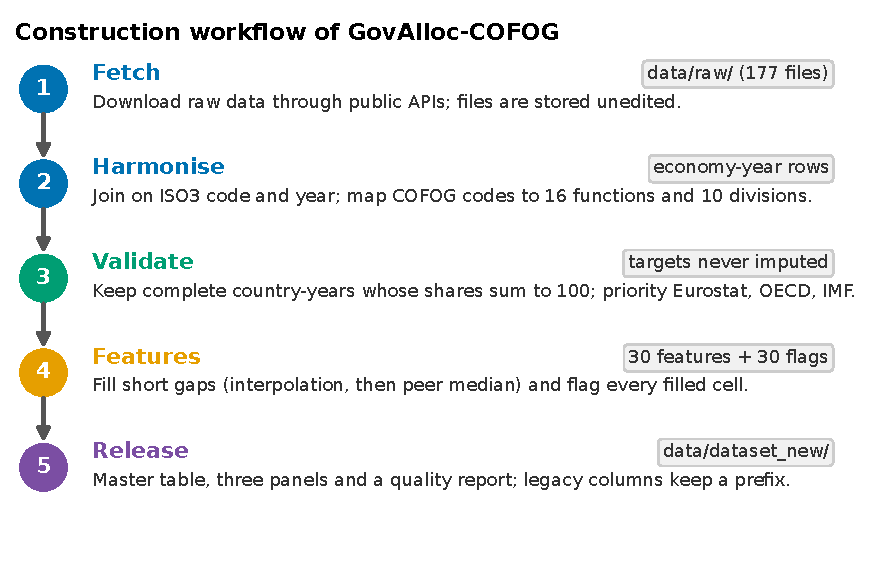
\includegraphics[width=0.93\linewidth]{figures/figD1_workflow.pdf}
\caption{Data construction workflow. Each stage is a script; raw downloads are never edited.}\label{fig:workflow}
\end{figure}

\subsection{Sources and access}
Table~\ref{tab:sources} lists the sources. Data were downloaded through public application programming interfaces (APIs) without registration or keys on 14 November 2026 (World Bank, Eurostat, OECD, IMF general-government COFOG); the IMF central-government extension and the two WGI institutional indicators were obtained through the APIs on 15 November 2026, and the fiscal-rule, election and IMF-programme files were downloaded manually from the providers' pages on the same day. Compilation used scripted API calls; code was developed with AI assistance (see the declaration at the end). Economy identifiers are the ISO~3166-1 alpha-3 codes used by the World Bank; Eurostat two-letter codes were mapped to them (Greece \texttt{EL} to \texttt{GR}), aggregates such as the euro area were dropped, and years are restricted to \DYearLo--\DYearHi. Region and income group are the World Bank labels at the time of access and are applied to all years, so an economy that changed class during the period is labelled with its current class.
\begin{table}[t]
\caption{Sources, content and terms of use. Terms were read from the providers' pages at the time of writing; verify them before redistribution (Section~\ref{sec:usage}).}\label{tab:sources}
\centering\small\renewcommand{\arraystretch}{1.1}
\begin{tabular}{@{}p{3.0cm}p{5.9cm}p{4.9cm}@{}}
\toprule
Source & Used for & Terms \\
\midrule
World Bank WDI~\cite{wdi}, WGI~\cite{kaufmann2011} & \DNumFeat{} features; four official sector series (Panel B); two extra WGI indicators in the institutional file & CC BY 4.0 (World Bank data terms) \\
Eurostat \texttt{gov\_10a\_exp}~\cite{eurostat_cofog} & COFOG groups and divisions, \DSixEconEs{} economies & Eurostat free-reuse policy with attribution \\
OECD National Accounts Table~11~\cite{oecd_table11} & COFOG for \DOecdAdded{} economies not in Eurostat, and overlap checks & OECD terms and conditions \\
IMF GFS COFOG~\cite{imf_gfs} & Ten divisions for non-EU/OECD economies (general government); central-government rows in the extended panel & IMF data terms of use \\
IMF Fiscal Rules Dataset, DPI 2020 (IADB), IMF MONA & Optional institutional covariates (file \texttt{institutional\_manual}) & Providers' terms; non-commercial research use \\
\bottomrule
\end{tabular}
\end{table}

\subsection{COFOG levels and the 16-function and 10-division targets}
COFOG has three levels: ten divisions (GF01 general public services, GF02 defence, GF03 public order and safety, GF04 economic affairs, GF05 environmental protection, GF06 housing and community amenities, GF07 health, GF08 recreation, culture and religion, GF09 education, GF10 social protection), groups (e.g.\ 04.5 transport) and classes. Publishers differ in the level they supply: Eurostat and the OECD publish groups, the IMF mainly divisions. We therefore define two target sets, both as percent of total general-government expenditure.
\begin{description}[leftmargin=1.2em,itemsep=2pt,parsep=0pt]
\item[A10 (ten divisions).] GF01--GF10 as published. The ten shares sum to 100 up to rounding.
\item[A16 (sixteen functions plus residual).] Eight divisions are used whole (GF01, GF02, GF03, GF05, GF07, GF08, GF09, GF10). Division 04 is split into agriculture (04.2), energy (04.3), industry and construction (04.4 and 04.7), transport (04.5), communication (04.6) and R\&D (04.8). Division 06 contributes water supply (06.3) and housing and community amenities (division 06 minus 06.3). The remaining economic-affairs groups (04.1 general economic affairs and 04.9 n.e.c.) form an explicit \emph{other/unallocated} residual, defined as 100 minus the sum of the 16 shares, so that all 17 components lie on the simplex. A compositional-data reading of the targets follows Aitchison~\cite{aitchison1986} and the log-ratio transformations of Egozcue et al.~\cite{egozcue2003}.
\end{description}
For the OECD, shares are computed with the sum of the ten published divisions as the denominator, so OECD and Eurostat shares are on the same base. No partial sums are formed: a share is missing if any required component is missing.

\subsection{Selection, consistency checks and source priority}
A country-year enters a COFOG panel only if \emph{all} its components exist (A16: \DSixIncomplete{} master rows with incomplete 16-function data are excluded from Panel A16 and flagged \texttt{cofog\_complete\_flag}=0). IMF series are accepted only when the raw ten divisions sum to between 97 and 103 and are then rescaled to sum to exactly 100; breakdowns outside this window (typically partial reporting) are discarded. When several sources cover the same country-year the order is Eurostat, then OECD, then IMF, and the chosen source is recorded in \texttt{cofog10\_source}. A companion file (\texttt{cofog10x}) adds \DTenXExtra{} country-years admitted under a relaxed window (raw sum 90--110, central-government scope for \DTenXCentral{} of them) with explicit scope and strictness flags; the strict panel A10 is unchanged by it.

\subsection{Feature set and imputation policy}
The \DNumFeat{} features are 26 WDI indicators and 4 WGI estimates (Table~\ref{tab:columns} and Fig.~\ref{fig:imp}): economic size and structure, demography, central-government fiscal aggregates, social and health indicators, infrastructure and environment, and governance. Gaps are filled in three ordered steps: (i) linear interpolation inside a country series across at most three consecutive missing years; (ii) edge fill (carrying the nearest value forward or backward) for at most three years; (iii) the median of the economy's region $\times$ income group $\times$ year cell. Each filled cell sets the flag \texttt{imp\_<feature>}=1 and the row-level count \texttt{n\_imputed\_features} is stored. \emph{Targets are never imputed.} Imputation is applied once to the full table, so interpolation can use later values and cell medians pool all economies; users who need strictly causal features should read the flags and recompute (Section~\ref{sec:usage}). Poverty headcount, the Gini index and adult literacy are structurally sparse (\DImpPov--\DImpLit\% of cells imputed) and are excluded from the 25 features used for modelling in the benchmark, but remain in the files with their flags. Two further WGI indicators (voice and accountability, political stability) and manually obtained institutional variables are provided as separate files keyed by \texttt{iso3} and \texttt{year}.

\subsection{Legacy dataset preservation}
The first version of the project used a dataset of \DLegacyRows{} rows for \DLegacyEcon{} economies and \DLegacyCols{} columns. It is kept verbatim in \texttt{dataset\_old/} and, so that it can be compared directly, all its columns are also in the master table with prefix \texttt{legacy\_}; country and year serve as keys and \DLegacyOnlyRows{} rows for Taiwan, which exist only in the legacy data, are marked \texttt{legacy\_only\_row}. Section~\ref{sec:legacy} documents its structure.

\section{Data Records}\label{sec:records}
\paragraph{Folder layout and formats.} The release (about \DDataTotalMB\,MB of processed files) is organised as \texttt{data/dataset\_new/} (processed GovAlloc-COFOG files), \texttt{data/dataset\_old/} (legacy) and \texttt{data/raw/} (verbatim downloads from World Bank, Eurostat, OECD, IMF and the institutional sources, \DRawFiles{} files). All processed files are UTF-8 comma-separated text with a header row, missing values empty, and one row per economy and year; the quality report is JSON. Descriptions of every file are in Table~\ref{tab:files}, and the column groups are summarised in Table~\ref{tab:columns}. A dataset card (\texttt{docs/guides/04\_dataset\_card.md}) accompanies the repository.
\begin{table}[t]
\caption{File inventory of GovAlloc-COFOG v1.0 (processed files; raw downloads are described in the text). Files in \texttt{dataset\_new/} start with \texttt{govalloc\_cofog\_} (omitted here), as does the legacy file in \texttt{dataset\_old/}. Rows $\times$ columns were counted from the files.}\label{tab:files}
\centering\footnotesize
\renewcommand{\arraystretch}{1.1}
\begin{tabular}{@{}p{4.4cm}p{4.9cm}rrr@{}}
\toprule
File & Content & Rows & Cols & Size \\
\midrule
\texttt{master.csv} & All economies $\times$ 2000--2024: features, flags, all targets, legacy columns & 5{,}450 & 217 & 5.68\,MB \\
\texttt{cofog\_panel.csv} & Panel A16: complete 16-function COFOG, Eurostat + OECD & 825 & 217 & 1.35\,MB \\
\texttt{cofog10\_panel.csv} & Panel A10: complete 10-division COFOG, Eurostat + OECD + IMF & 1{,}526 & 217 & 2.22\,MB \\
\texttt{cofog10x\_panel.csv} & A10 plus rows admitted under a relaxed rule (scope/strictness flags) & 1{,}539 & 221 & 2.27\,MB \\
\texttt{wdi\_panel.csv} & Panel B: rows with at least one official WDI sector series & 4{,}995 & 217 & 5.32\,MB \\
\texttt{institutional\_features.csv} & WGI voice \& accountability, political stability (+ 2-year changes) & 4{,}903 & 6 & 317\,kB \\
\texttt{institutional\_manual.csv} & Fiscal rules, election timing, IMF programme indicators & 9{,}119 & 10 & 279\,kB \\
\texttt{data\_quality.json} & Coverage, imputation, cross-source and legacy audit statistics & -- & -- & 7\,kB \\
\texttt{legacy\_dataset.csv} & Legacy dataset, verbatim (semi-synthetic sectors); in dataset\_old/ & 775 & 59 & 543\,kB \\
\bottomrule
\end{tabular}
\end{table}

\begin{table}[t]
\caption{Column dictionary of the master table (\DMasterCols{} columns); the three modelling panels contain the same columns.}\label{tab:columns}
\centering\small
\renewcommand{\arraystretch}{1.12}
\begin{tabular}{@{}p{3.6cm}rp{9.4cm}@{}}
\toprule
Group & Columns & Content \\
\midrule
Identifiers and groupings & 6 & \texttt{iso3}, \texttt{iso2}, \texttt{country}, \texttt{region}, \texttt{income\_group} (World Bank, current classification), \texttt{year} \\
Socio-economic features & 30 & 26 WDI and 4 WGI indicators (GDP, inflation, demography, fiscal, health, infrastructure, governance); \texttt{units in column name} \\
Imputation flags & 30 & \texttt{imp\_<feature>} = 1 if the cell was filled, 0 if observed \\
WDI sector targets & 7 & education, domestic government health, military (each \% of GDP and of government expenditure) and R\&D (\% of GDP), observed only \\
Derived fields & 5 & \texttt{n\_imputed\_features}, \texttt{log\_gdp}, \texttt{log\_pop}, \texttt{has\_legacy\_v1\_row}, \texttt{wdi\_target\_n} \\
COFOG-16 targets, share of total & 17 & 16 functions plus an explicit residual, \% of general-government expenditure (the simplex targets of panel A16) \\
COFOG-16, share of GDP & 17 & same functions as \% of GDP (Eurostat and OECD) \\
COFOG-16, national currency & 17 & same functions plus total, million euro (Eurostat only) \\
COFOG-16, derived USD & 16 & share of GDP $\times$ World Bank GDP in current USD (derived, not an official figure) \\
COFOG-16 provenance & 3 & \texttt{cofog\_complete\_flag}, \texttt{cofog\_source\_name}, \texttt{cofog\_source} \\
COFOG-10 targets & 10 & divisions GF01--GF10, \% of total expenditure (panel A10) \\
COFOG-10 provenance & 2 & \texttt{cofog10\_source} (Eurostat / OECD / IMF), \texttt{cofog10\_complete\_flag} \\
Legacy columns & 57 & all 57 legacy columns with prefix \texttt{legacy\_} (semi-synthetic sector columns; see Section~\ref{sec:legacy}); \texttt{legacy\_only\_row} marks the Taiwan rows \\
\midrule
Total & 217 & \\
\bottomrule
\end{tabular}
\end{table}


\paragraph{Panels.} \emph{Panel A16} (\DRowsSix{} country-years, \DEconSix{} economies; \DSixRowsEs{} Eurostat and \DSixRowsOecd{} OECD rows) holds the 16 functions plus residual. \emph{Panel A10} (\DRowsTen{} country-years, \DEconTen{} economies) comes from Eurostat (\DTenRowsEs{} rows, \DTenEconEs{} economies), the OECD (\DTenRowsOecd{} rows, \DTenEconOecd{} economies) and the IMF (\DTenRowsImf{} rows, \DTenEconImf{} economies). The median economy has \DTenYrsMedian{} years of data, but \DTenShortN{} economies have fewer than ten and the shortest has \DTenYrsMin. \emph{Panel B} (\DRowsWdi{} country-years, \DEconWdi{} economies) contains rows with at least one of the seven official WDI sector series; \DWdiSixPlus{} rows have six or seven of them and \DWdiOneTwo{} have one or two.

\paragraph{Coverage.} Table~\ref{tab:coverage} and Figs.~\ref{fig:years} and~\ref{fig:groups} show coverage over time, income group and region. Coverage is not uniform and should be considered before pooling (Section~\ref{sec:usage}): A16 contains \DEconSixHi{} high-income economies and one upper-middle-income economy (Colombia), A10 reaches \DEconTenUm{} upper-middle, \DEconTenLm{} lower-middle and only \DEconTenLo{} low-income economies (Afghanistan, Somalia and Yemen), whereas Panel B covers \DEconWdiLo{} low-income economies but only for four functions.
\begin{table}[t]
\caption{Coverage by World Bank income group (current classification applied to all years): economies (country-years) in each file. A10 covers 85 economies but only \DEconTenLo{} low-income and \DEconTenLm{} lower-middle-income ones.}\label{tab:coverage}
\centering\small
\begin{tabular}{@{}lrrrr@{}}
\toprule
Income group & Master & Panel B (WDI) & Panel A10 & Panel A16 \\
\midrule
High income & 86 (2{,}150) & 80 (1{,}781) & 50 (1{,}064) & 35 (809) \\
Upper middle income & 59 (1{,}475) & 59 (1{,}458) & 23 (371) & 1 (16) \\
Lower middle income & 47 (1{,}175) & 47 (1{,}167) & 9 (61) & 0 (0) \\
Low income & 25 (625) & 25 (589) & 3 (30) & 0 (0) \\
\midrule
All & 217 (5{,}425) & 211 (4{,}995) & 85 (1{,}526) & 36 (825) \\
\bottomrule
\end{tabular}
\end{table}

\begin{figure}[t]
\centering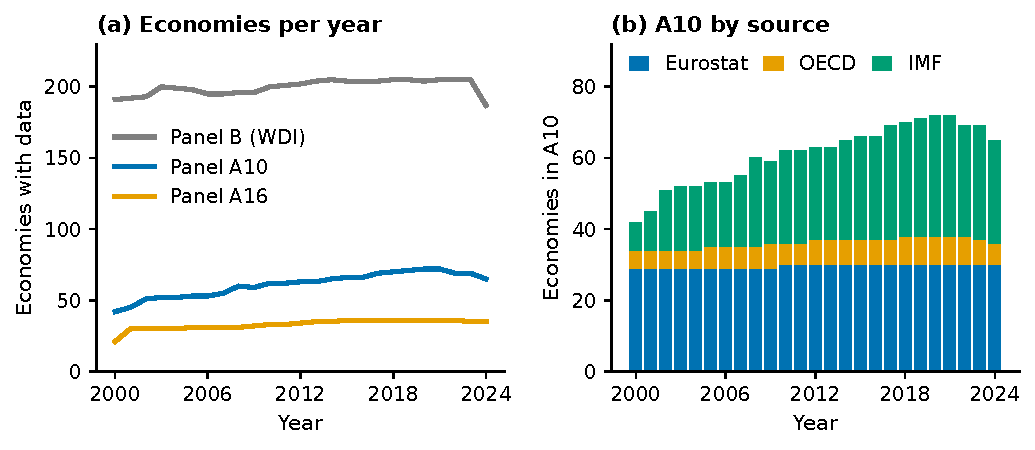
\includegraphics[width=\linewidth]{figures/figD2_coverage_years.pdf}
\caption{Coverage over time. (a) Economies with data per year in each panel (the fall of Panel B in 2024 probably reflects publication lags of WDI series). (b) Panel A10 economies by source.}\label{fig:years}
\end{figure}
\begin{figure}[t]
\centering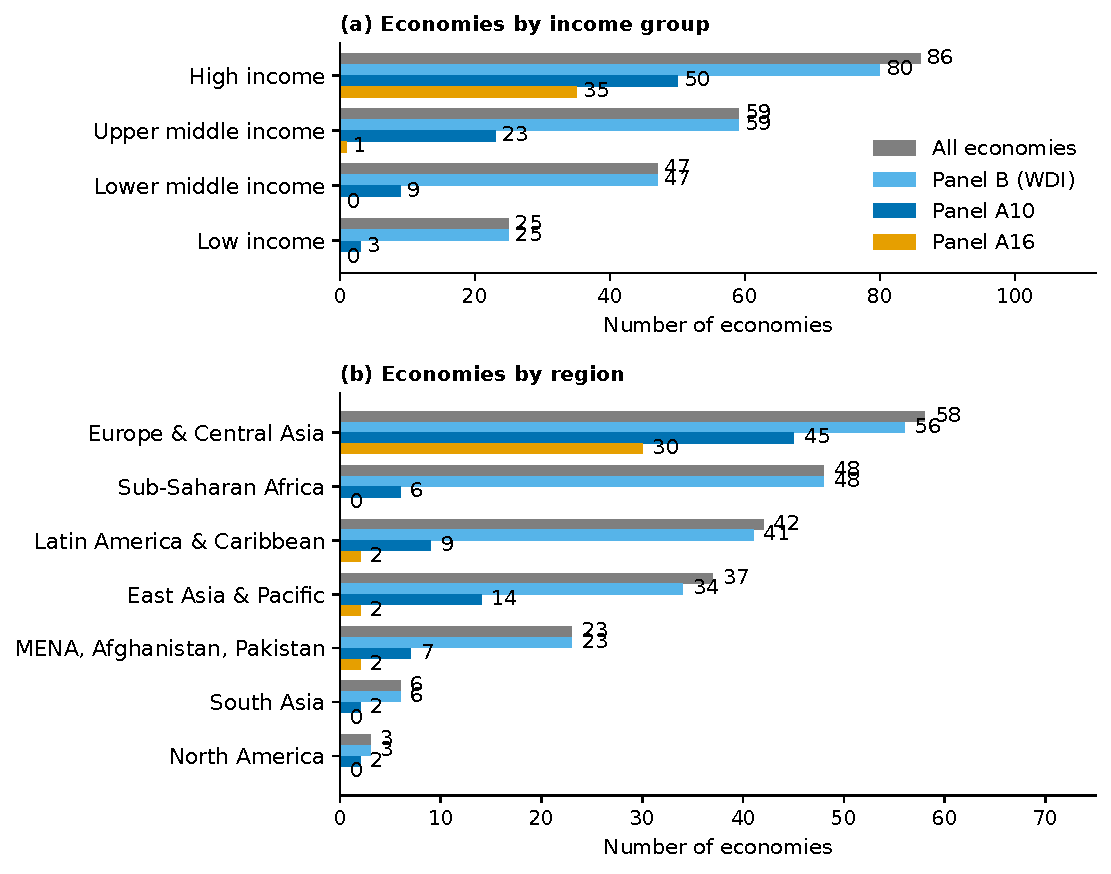
\includegraphics[width=0.95\linewidth]{figures/figD5_coverage_groups.pdf}
\caption{Number of economies by World Bank income group and by region for the master table (official-data economies), Panel B, Panel A10 and Panel A16.}\label{fig:groups}
\end{figure}

\paragraph{Versioning and persistent identifier.} The current version is v1.0 of GovAlloc-COFOG; version history is in the Git repository. The earlier project dataset is called the \emph{legacy} dataset throughout. The release is archived on Zenodo with a permanent identifier: \url{https://doi.org/10.5281/zenodo.24248315} (concept DOI, always resolves to the latest version) and \url{https://doi.org/10.5281/zenodo.24248316} (version 1.0). Companion code and the benchmark paper cite the same release.

\section{Technical Validation}\label{sec:validation}
Table~\ref{tab:checks} summarises the automated checks; all are recomputed from the released files by \texttt{pipeline/28\_dataset\_paper\_figures.py}. We discuss them in turn.
\begin{table}[t]
\caption{Summary of automated validation checks (all computed by \texttt{pipeline/28\_dataset\_paper\_figures.py} from the released files).}\label{tab:checks}
\centering\small
\renewcommand{\arraystretch}{1.1}
\begin{tabular}{@{}>{\raggedright\arraybackslash}p{3.8cm}>{\raggedright\arraybackslash}p{3.2cm}>{\raggedright\arraybackslash}p{7.8cm}@{}}
\toprule
Check & Scope & Result \\
\midrule
Component shares sum to 100 & A16, 825 rows & maximum deviation $\DSumSixMaxDev$ pp \\
Component shares sum to 100 & A10, 1{,}526 rows & Eurostat rows 99.7--100.3 (published rounding); OECD and IMF rows exactly 100 \\
Missing targets & A16, A10 & 0 and 0 missing cells (complete-case panels; targets never imputed) \\
Negative values & A16, A10 & 27 of 14{,}025 A16 cells (25 country-years), 11 A10 cells; minimum -3.8 pp; kept as published \\
Upper bounds & A16, A10 & largest share 47.0\% (social protection); no share above 100\% \\
Duplicate \texttt{iso3}--\texttt{year} keys & master and three panels & 0 duplicates; all years in 2000--2024 \\
Eurostat vs OECD & 690 country-years, 15 functions & median $|\Delta|$ 0.023--0.028 pp; $r\ge0.964$ \\
IMF vs Eurostat & 723 country-years, 10 divisions & median $|\Delta|$ 0.027--0.062 pp; $r\ge0.984$ \\
COFOG vs WDI sector series & A10, health / education / defence & $r=$0.82 / 0.76 / 0.79 (different definitions) \\
Year-to-year jumps & A10, 1{,}426 consecutive pairs & 98 (6.9\%) move more than 10 pp (total variation); flagged by users, not removed \\
WDI series bounds & Panel B & 0 negative values; no \%-of-expenditure value above 100 \\
Legacy features vs World Bank & 750 legacy rows & identical for 6 of 7 checked indicators; inflation within 0.4\% on 90\% of rows \\
\bottomrule
\end{tabular}
\end{table}


\subsection{Internal consistency: sums, bounds and negative values}
In A16 the 17 components sum to 100 to within $\DSumSixMaxDev$ pp by construction (the residual closes the vector). In A10 the Eurostat rows sum to between \DSumTenEsMin{} and \DSumTenEsMax{} because the publisher rounds each division to one decimal, while OECD and IMF rows sum to 100 exactly after our normalisation. There are no missing targets in the complete-case panels and no duplicate \texttt{iso3}--\texttt{year} keys. No share exceeds 100\%; the largest is \DSixMax\% (social protection in A16). Negative values do occur: \DNegSix{} of \DNegSixCells{} A16 cells (in \DNegSixRows{} country-years), concentrated in communication (\DNegSixComm) and housing and community amenities (\DNegSixHous), plus one negative residual (\DNegSixResMin\,pp, Luxembourg 2001), and \DNegTen{} A10 cells (minimum \DTenNegMin\,pp). They are kept as published or derived because a negative sub-function can reflect net receipts or a difference of two published series; users who need strictly non-negative compositions should clip and renormalise, or exclude the affected rows, and report the choice.

\subsection{Cross-source agreement}
Where two sources publish the same quantity we can test our harmonisation (Fig.~\ref{fig:cross}). On the \DEoN{} country-years that Eurostat and the OECD both report, the median absolute difference of a function's share lies between \DEoMedLo{} and \DEoMedHi{} pp and Pearson's $r$ is at least \DEoRminB{} for every function except communication ($r=\DEoRmin$, a small function). IMF ten-division shares agree with Eurostat on \DIeN{} overlapping country-years with median absolute differences of \DIeMedLo--\DIeMedHi{} pp and $r\ge\DIeRmin$, the weakest being general public services. The residual differences are small enough to be consistent with rounding and with revisions between data vintages (we did not investigate them individually) and were not adjusted.\begin{figure}[t]
\centering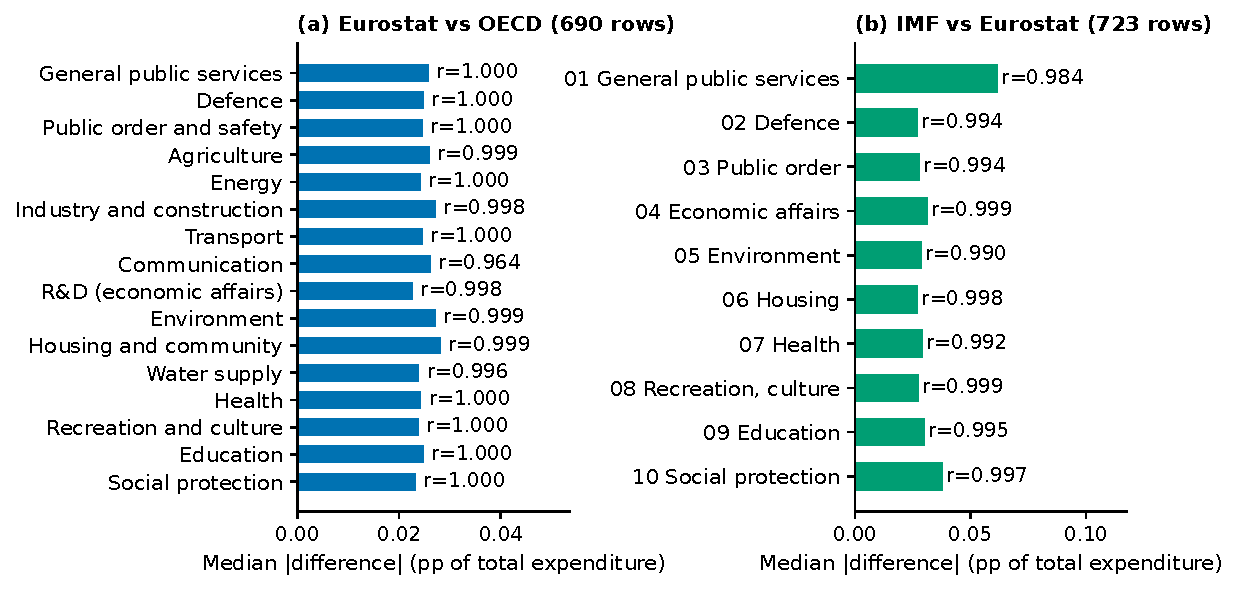
\includegraphics[width=\linewidth]{figures/figD3_cross_source.pdf}
\caption{Cross-source agreement: median absolute difference in percentage points of total expenditure, with Pearson's $r$ printed beside each bar. (a) Eurostat vs OECD, 15 functions (the residual is derived, not published). (b) IMF vs Eurostat, ten divisions.}\label{fig:cross}
\end{figure}
For construct validity we compare COFOG shares with the independently defined WDI shares of government expenditure on the same function. They differ in definition, so only association is expected: Pearson $r$ is \DCvRHealth{} for health (GF07 vs.\ domestic general-government health, $n=\DCvNHealth$), \DCvREdu{} for education ($n=\DCvNEdu$) and \DCvRDef{} for defence ($n=\DCvNDef$), with median absolute gaps of \DCvMedHealth, \DCvMedEdu{} and \DCvMedDef{} pp.

\subsection{Outliers and breaks}
Between consecutive years the median change in the allocation of A10 (total-variation distance) is \DJumpMed{} pp, but \DJumpN{} of \DJumpTot{} pairs (\DJumpPct\%) move by more than 10 pp (maximum \DJumpMax{} pp), in \DJumpEcon{} economies. \DJumpImf{} of these involve IMF-sourced rows, whose series for developing economies are often short; only \DJumpCovid{} fall in 2020. We neither remove nor smooth them: they may be genuine fiscal shocks, reclassifications or reporting changes, and a \texttt{cofog10\_source} column allows users to treat them separately.

\subsection{Missingness, imputation and coverage}
Among the \DMasterEconYears{} official-data economy-years, an average feature has \DImpMean\% of its cells imputed and \DMissMean\% still missing afterwards; the worst is \DMissMaxName{} (\DMissMax\% missing). Imputation is heavily concentrated: \DImpGtFifty{} features have more than half of their cells imputed (poverty, Gini, adult literacy, central-government debt) and the four fiscal series from the World Bank's central-government tables lie at \DImpFiscalLo--\DImpFiscalHi\%, whereas \DImpLtFive{} features have under 5\% (Fig.~\ref{fig:imp}). The WGI estimates are \DImpWgiLo--\DImpWgiHi\% imputed. The rows that enter the modelling panels are better covered: on average \DImpRowSix{} features are imputed per A16 row and \DImpRowTen{} per A10 row (\DImpCellsSix\% and \DImpCellsTen\% of cells), probably because the economies with COFOG data are better documented. Imputation shares by income group are \DImpIncHi\% (high), \DImpIncUm\% (upper-middle), \DImpIncLm\% (lower-middle) and \DImpIncLo\% (low), so imputation is a poor proxy for data quality and the flags should be used directly. Coverage by income group and region (Table~\ref{tab:coverage}, Fig.~\ref{fig:groups}) is the main structural limitation.
\begin{figure}[t]
\centering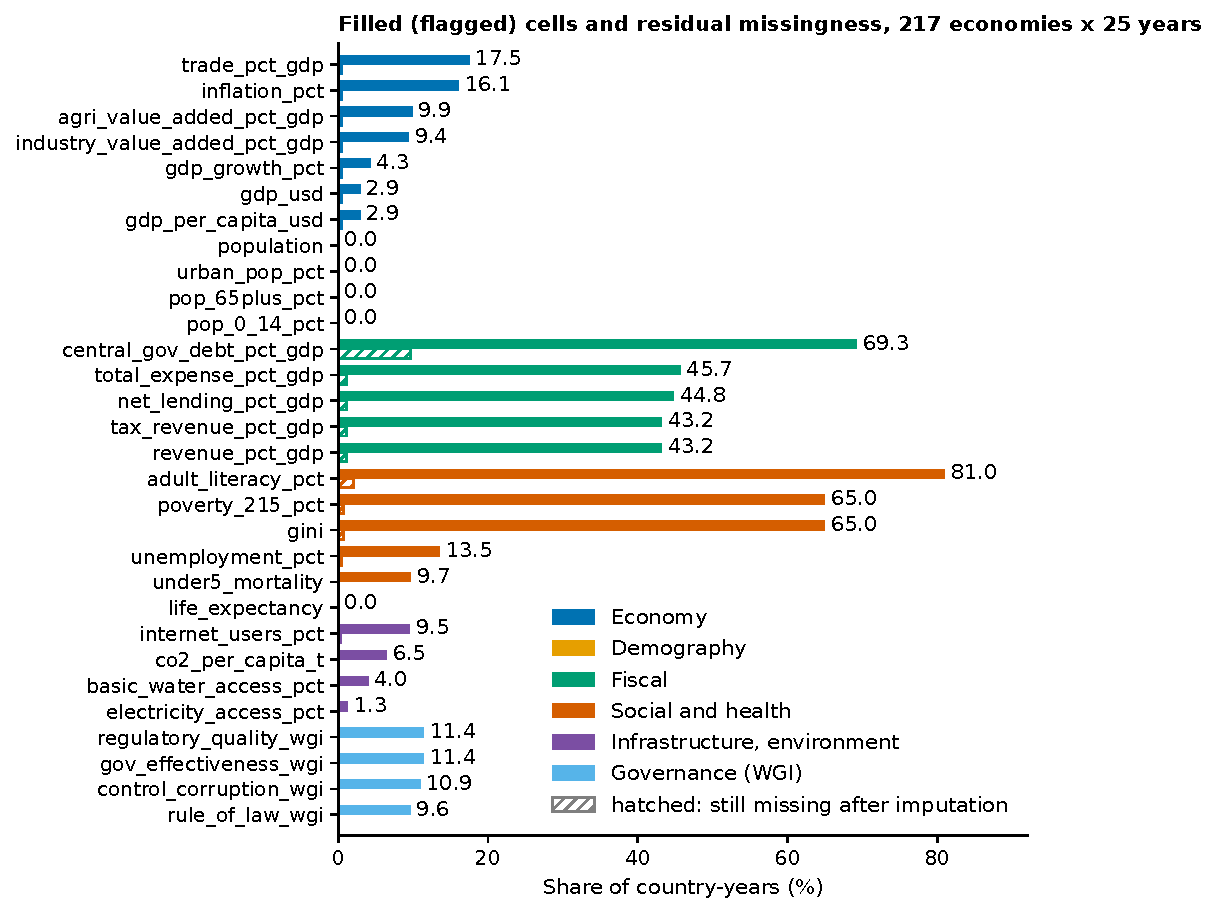
\includegraphics[width=0.93\linewidth]{figures/figD4_imputation.pdf}
\caption{Share of cells filled by the imputation rule (solid bars, labelled) and share still missing (hatched) for each of the 30 features, grouped by theme. Values are for the \DMasterEcon{} economies with official data.}\label{fig:imp}
\end{figure}
The build script's JSON report states the missing shares over all \DMasterRows{} master rows, including the \DLegacyOnlyRows{} legacy-only Taiwan rows, which carry no features; this accounts for the small difference to the figures above.

\subsection{Legacy dataset: why it must not be used}\label{sec:legacy}
The legacy file is retained because the earlier benchmark results were published on it and users may encounter it, but our audit shows that its sector columns are not real allocation data. \DLegMult{} of its fifteen sector columns are exact fixed multiples of one series: relative to the agriculture column the ratios take the values $0.5$ to $3.0$ and their standard deviation across all \DLegacyRows{} rows is below $\DLegRatioSdMax$. All rows therefore share one identical mix among these sectors (\DLegMixes{} distinct mix); only their total ($\approx\DLegLatentMean\%$ of GDP, SD \DLegLatentSd\,pp) varies, and it correlates $r=\DLegCorrGrowth$ with GDP growth. A one-parameter rule ``constant multiple of GDP'' reproduces these columns almost perfectly: on a random 80/20 split, gradient boosting reaches $R^2=\DBmLegXGBRConst$ and the rule \DBmLegFormulaRConst{} (USD scale), while a constant share of GDP scores $R^2=\DBmLegConstRatioConst$ on the share scale; the headline mean $R^2=\DBmLegXGBR$ is therefore driven by economic scale, not allocation. In addition, \DLegIdent{} column pairs are identical (\DLegIdentTargets{} involve a target), including every SDG ``budget'' with its parent sector, and the legacy health column is the same as an input feature, a form of target leakage~\cite{kaufman2012,kapoor2023}. Only a few legacy columns relate to real statistics: education and R\&D match the WDI series to machine precision, defence matches it ($r=\DLegDefR$), but healthcare differs from the official domestic government health series (median gap \DLegHealthGap\,pp, $r=\DLegHealthR$). Its \emph{features} do match the World Bank values (identical for \DLegExactFeat{} of the seven indicators we compared on \DLegFeatN{} rows; inflation within \DLegInflPninety\% on 90\% of rows). We therefore treat the legacy file as semi-synthetic: its features are real, its sector columns are not, and it is \emph{not recommended for modelling}.

\subsection{Benchmark summary}
The panels support the benchmark study~\cite{govallocxai_benchmark}; the numbers below are quoted from it. With a temporal split on A16, last year's allocation (persistence) has a total-variation distance of \DBmResTVDPersist{} pp (95\% CI \DBmResTVDPersistLo--\DBmResTVDPersistHi); a learned same-year-covariate correction lowers it to \DBmResTVDHyb{} pp, a gain of \DBmResPairedGain{} pp (CI \DBmResPairedLo--\DBmResPairedHi) that is significant for only \DBmAnnSeedNExcl{} of \DBmAnnSeedN{} learner seeds. Persistence is thus a strong baseline that every user of the data should report. For economies with no history (leave-country-out), a stacked learner reaches \DBmColdStackTen{} pp against \DBmColdPeerTen{} pp for the income-group mean on A10 (and \DBmColdStackSixteen{} against \DBmColdPeerSixteen{} on A16); errors are largest for low-income economies (\DBmErrLow{} pp against \DBmErrHigh{} pp for high income, with only three low-income economies, hence exploratory). These results show that the panels are informative but that gains over simple baselines are modest, as one would expect from real data.

\section{Usage Notes}\label{sec:usage}
\paragraph{Loading.} The files are plain CSV.
\begin{verbatim}
import pandas as pd
a10 = pd.read_csv(
    "data/dataset_new/govalloc_cofog_panel_a10.csv")
a10["region"] = a10["region"].str.strip()   # trailing blanks
Y = a10.filter(regex=r"^cofog10_GF\d\d_pct_total$")  # 10 shares
X = a10[["log_gdp", "gdp_growth_pct", "gov_effectiveness_wgi"]]
\end{verbatim}
\begin{verbatim}
a10 <- read.csv(
  "data/dataset_new/govalloc_cofog_panel_a10.csv")
y <- a10[, grep("^cofog10_GF[0-9]{2}_pct_total$",
                names(a10))]
\end{verbatim}
\paragraph{Splits and pitfalls.}
\begin{itemize}[leftmargin=1.4em,itemsep=1pt,parsep=0pt]
\item \emph{Group by economy.} Rows of the same economy are strongly dependent (median year-to-year change is \DJumpMed{} pp). Use leave-country-out or leave-region-out cross-validation when the aim is to generalise to unseen economies~\cite{roberts2017}, and temporal splits when the aim is to forecast.
\item \emph{No future leakage.} Imputed features were filled by interpolation and cell medians that use later years and other economies. For a forecasting study, mask cells with \texttt{imp\_*}=1 or recompute the fill using only past data. Lags of targets must come from earlier years only.
\item \emph{Executed versus approved spending.} Targets are outturn statistics for general government, not budget proposals; they are published with a delay and are revised.
\item \emph{COFOG levels differ.} A16 and A10 have different numbers of components, so distances between them are not comparable; A16 mixes divisions and groups and has an explicit residual. IMF rows are general government unless the extended file flags central government.
\item \emph{Source mix.} Source and classification can change a series' level; include \texttt{cofog10\_source} in diagnostics, particularly for the IMF rows with large jumps.
\item \emph{Always report a persistence and an income-group mean baseline.} The gains of learners over them are small (Section~\ref{sec:validation}).
\item \emph{Do not model the legacy columns.} Use them only for audits, such as reproducing Section~\ref{sec:legacy}.
\end{itemize}
\paragraph{Licensing and attribution.} The code and our compilation scripts are released under the MIT licence (\texttt{LICENSE} in the repository). The data are compiled from third-party sources whose terms (Table~\ref{tab:sources}) continue to apply to the derived values: users should cite the original publishers (World Bank, Eurostat, OECD, IMF) together with this dataset, and should check the current OECD and IMF terms (and those of the institutional files) before redistributing derived rows. A dataset-level licence for the Zenodo record will be chosen to be consistent with the most restrictive source terms; until then the files are provided for research and teaching use with attribution.
\paragraph{Ethical statement.} All data are aggregated national statistics about governments; no personal data were collected and no ethics approval was required. Panels describe public spending, not the welfare of individuals, and conclusions about a country should not be drawn from a single year or from a model without checking data quality flags. Models built on these data should support analysis, not decide funding.
\paragraph{Limitations.} (i) Coverage is centred on Europe and the OECD: \DEconSix{} economies in A16 (\DSixNonHigh{} not high-income) and a low-income count of \DEconTenLo{} in A10. (ii) Income group and region are the current World Bank classes applied to all years. (iii) The 16-function taxonomy is an analytical mapping, not an official classification, and its residual averages \ResidualMean\% of expenditure (maximum \ResidualMax\%). (iv) Feature imputation is transductive (Section~\ref{sec:methods}), and several fiscal features are more than 40\% imputed. (v) IMF series for developing economies are short and sometimes revised, and general-government scope is not fully uniform across sources. (vi) Executed spending hides arrears, off-budget items and sub-national differences that are outside general-government totals. (vii) The extended file mixes strictly consistent and relaxed rows; use the flags.

\section{Code and Data Availability}
\paragraph{Data.} The files described here are in the \texttt{data/} folder of the public repository \url{https://github.com/Pranav-chaudhari-2006/GovAllocXAI}; the permanent archive and its identifier are given in Section~\ref{sec:records}. All raw inputs are public (Table~\ref{tab:sources}).

\paragraph{Code.} The fetching, building and checking scripts (\texttt{pipeline/01}--\texttt{03}, \texttt{14}, \texttt{23}--\texttt{24}, \texttt{28}), the dataset card and the audits are in the same repository (MIT licence). Re-running \texttt{pipeline/01}, \texttt{02} and \texttt{03} rebuilds the processed files from fresh downloads; because the providers revise data, a rebuild will not be identical to this release, which is why the raw files are archived.

\section*{Authors' Contribution and CRediT}
\noindent Conceptualization: A.H.J., P.S.C.\\
\noindent Methodology: A.H.J., P.S.C., D.P.B.\\
\noindent Software: P.S.C., D.P.B.\\
\noindent Validation: G.M.J., D.P.B.\\
\noindent Formal analysis: P.S.C., G.M.J.\\
\noindent Investigation: G.M.J., A.H.J.\\
\noindent Resources: G.M.J.\\
\noindent Data curation: P.S.C., G.M.J.\\
\noindent Writing---original draft: P.S.C., G.M.J.\\
\noindent Writing---review \& editing: all authors\\
\noindent Visualization: D.P.B., P.S.C.\\
\noindent Supervision and project administration: A.H.J.

\medskip\noindent\textbf{Author abbreviations:}\par
\noindent Pranav S.\ Chaudhari (P.S.C.),\\
\noindent Aditi H.\ Joshi (A.H.J.),\\
\noindent Gaurav M.\ Jaypatre (G.M.J.),\\
\noindent Digvijay P.\ Birajdar (D.P.B.)

\section*{Competing interests}
All authors have reviewed the manuscript and declare that they have no known competing financial interests or personal relationships that could have appeared to influence the work reported in this paper.

\section*{Funding}
This research received no external funding.

\section*{Declaration of generative AI and AI-assisted technologies in the manuscript preparation process}
During the preparation of this work the authors used Anthropic's Claude, an AI coding and writing assistant, for code scaffolding, the data-collection and data-building scripts (which call the public APIs listed above), drafting and editing of text, and for simulated critical review of the manuscript. The legacy dataset described in Section~\ref{sec:legacy} had itself been partly populated with the help of a large language model, which is the reason for its semi-synthetic structure. All numbers in this paper are computed from the released files by script. The authors reviewed and edited all content produced with these tools and take full responsibility for the content of the publication.

\section*{Acknowledgements}
The authors thank the Department of Computer Engineering, Pimpri Chinchwad College of Engineering, Pune, for computing resources.

{\small\bibliographystyle{IEEEtran}
\bibliography{references}}
\end{document}
